\documentclass[10pt,twocolumn,letterpaper]{article}

\usepackage{cvpr}
\usepackage{times}
\usepackage{epsfig}
\usepackage{graphicx}
\usepackage{amsmath}
\usepackage{amssymb}
\usepackage{algorithm}
%\usepackage[backend=biber]{biblatex}
%\usepackage{algpseudocode}


% Include other packages here, before hyperref.

% If you comment hyperref and then uncomment it, you should delete
% egpaper.aux before re-running latex.  (Or just hit 'q' on the first latex
% run, let it finish, and you should be clear).
\usepackage[pagebackref=true,breaklinks=true,letterpaper=true,colorlinks,bookmarks=false]{hyperref}

% \cvprfinalcopy % *** Uncomment this line for the final submission

\def\cvprPaperID{****} % *** Enter the CVPR Paper ID here
\def\httilde{\mbox{\tt\raisebox{-.5ex}{\symbol{126}}}}

% Pages are numbered in submission mode, and unnumbered in camera-ready
\ifcvprfinal\pagestyle{empty}\fi

\begin{document}

%%%%%%%%% TITLE
\title{A-Lamp: Adaptive Layout-Aware Multi-Patch Deep Convolutional Neural Network for Photo Aesthetic Assessment}

\author{First Author\\
Institution1\\
Institution1 address\\
{\tt\small firstauthor@i1.org}
% For a paper whose authors are all at the same institution,
% omit the following lines up until the closing ``}''.
% Additional authors and addresses can be added with ``\and'',
% just like the second author.
% To save space, use either the email address or home page, not both
\and
Second Author\\
Institution2\\
First line of institution2 address\\
{\tt\small secondauthor@i2.org}
}

\maketitle
%\thispagestyle{empty}
%%%%%%%%% ABSTRACT
\begin{abstract}	
		
Deep convolutional neural networks (CNN) have recently been shown to generate promising results for aesthetics assessment. However, the performance of these deep CNN methods is often compromised by the constraint that the neural network only takes the fixed-size input. To accommodate this requirement, input images need to be transformed via cropping, wrapping, or padding, which often alter image composition, reduce image resolution, or cause image distortion. Thus the aesthetics of the original images is impaired because of potential loss of fine grained details and holistic image layout. However, such fine grained details and holistic image layout is critical for evaluating an image’s aesthetics. 
In this paper, we present an Adaptive Layout-Aware Multi-Patch Convolutional Neural Network (A-Lamp CNN) architecture for photo aesthetic assessment. This novel scheme is able to accept arbitrary sized images, and learn from both fined grained details and holistic image layout simultaneously. To support A-Lamp training on these hybrid inputs, we extend the method by developing a dedicated double-subnet neural network structure, i.e. a Multi-Patch subnet and a Layout-Aware subnet. We further construct an aggregation layer to effectively combine the hybrid features from these two subnets. Extensive experiments on the large-scale aesthetics assessment benchmark (AVA) demonstrate significant performance improvement over the state of the art in photo aesthetic assessment.

\end{abstract}

%%%%%%%%% BODY TEXT
\section{Introduction} \label{intro}

\begin{figure}
	\centering
	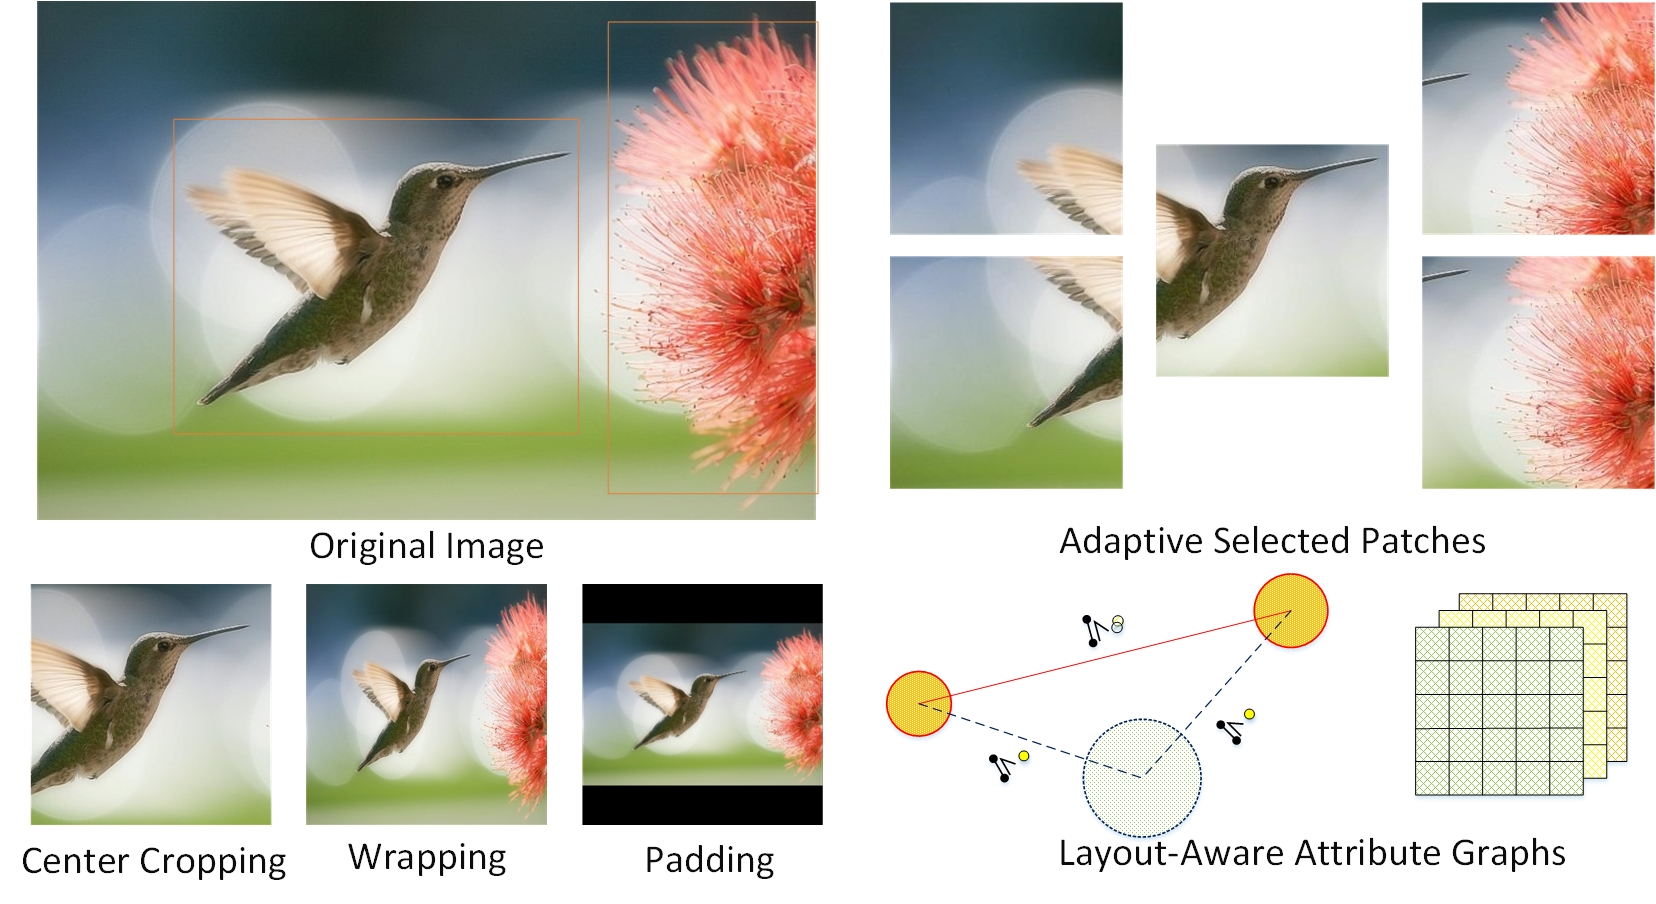
\includegraphics[scale=0.25]{figures/intro}
	\label{transform}
	\caption{Illustration fo image transformation.}
\end{figure}
%%%%%%% Potential Application%%%%%%%%%%%%
Problems of image aesthetics assessment 
have drawn numerous research attentions with the goal of 
endow computers with the capability of perceiving aesthetics and
visual quality as human vision systems. Potential usage for this task could be foreseen towards wide contemporary applications from intelligent computer
systems to real-time, mobile applications. 

%%%%%%% previous hand-craf work%%%%%%%%%%%%
However, assessing photo aesthetics is challenging. 
Early methods \cite{Datta:2006:ECCV,Ke:2006:CVPR} manually design various hand-craft aesthetics features to approximate a number of photographic and psychological aesthetics rules, including low-level features \cite{Luo:2008:ECCV,Bhattacharya:2010:ACMMM} (distribution of edges, color histograms and light contrast, etc.), as well as high level features \cite{Tang:2013:TMM,Sagnik:2011:CVPR,Su:2011:ACMMM,Cohen-Or:2006:SIGGRAPH} (composition principles, e.g. "Rule of Thirds", "Visual Balance" and "Golden Ratio", Low-of-Depth, color harmony, photo content and scene categories, etc.). 
Although these handcraft features have shown encouraging 
results. Manually design effective aesthetics features is still a challenging task because even experienced photographers use very abstract terms to describe high quality photos.
%%%%% generic feautres 
Other approaches have been developed to leverage more generic image features, such as SIFT, Fisher Vector 
\cite{Marchesotti:2011:ICCV,Perronnin:2010:ECCV} and bag of visual words \cite{Su:2011:ACMMM}, to predict photo aesthetics. Though obtaining
promising performance, the image representation provided
by those generic features may not be optimal for the 
task of photo aesthetics, as they are designed to represent natural images in
general, not specifically for aesthetics assessment.

%%%%% CNN method %%%%%%%%%%%%%%%
Because of these limitations, many researchers are attempting to use deep learning methods to extract effective aesthetics features \cite{Lu:2015:ICCV,Lu:2014:ACMMM,Mai:2016:CVPR,Tang:2014:CVPR,Karaye:2013:Archive:style}. Although these deep CNN methods have shown promising results, the performance is often compromised by the constraint that the neural network only takes the fixed-size input. To accommodate this requirement, input images need to be transformed via cropping, wrapping, or padding. These operations often alter image composition, reduce image resolution, or cause image distortion, and thus impair the aesthetics of the original images because of potential loss of fine grained details and holistic image layout. However, such fine-grained details and image layout have been shown highly useful in many applications such as image quality estimation \cite{Kang:2014:CVPR,DBLP:2016:img_quality_assessment}, image aesthetics categorization\cite{Lu:2014:ACMMM,2010:ICIP:composition,2010:optimizing_composition,2012:ICIP:composition,ICML:2012:composition,Zhou:2015:ACMMM:vanishing_point}, and image style classification \cite{Karaye:2013:Archive:style,Gatys:2016:CVPR:style_transfer}. 
As we can see from Fig.\ref{transform}, one randomly cropped patch may generate ambiguity in training examples as aesthetic attributes in one patch may not well represent the holistic information in the entire image (the flower is eliminated and only the bird is remained). Uniformly wrapping reduces original image resolution and distorts the salient object thus compromises the detail clarity of the important regions. The artificial boundaries between the original image and the padding area could possibly confuse the neural network. Finally, training from such transformed images will likely make the data more ambiguous and thus compromise the ability of the network to learn effective discriminative features.

%%%%%%% SPP and CVPR'16 solve fixed-size strategy%%%%%%%%%%%
Some works address the fixed-size restriction by training images in a few different scales to mimic varied input sizes \cite{He:archive:2014,Mai:2016:CVPR}. However, they still learn from transformed images, which may result in loss of fine grained details and distortion of image layout. To support learning from fine-grained details, \cite{Lu:2015:ICCV} proposed a deep multi-patch aggregation network architecture (DMA-Net) to take multiple random cropped patches as input. This network shows promising results. However, these orderless bag of patches cannot represent image layout, which result in the global information missing. Moreover, the random cropping strategy requires a large number of training epochs, which lead to very low efficiency.

To resolve the above mentioned issues, we present an Adaptive Layout-Aware Multi-Patch Convolutional Neural Network (A-Lamp CNN) architecture for photo aesthetic assessment. This dedicated CNN can accept arbitrary image sizes, and deal with both the fine-grained details as well as image layout simultaneously.
Learning from fine grained details is achieved by constructing multiple, shared columns in a Multi-Patch subnet and feeding multiple patches to each of the columns. Instead of conventional random cropping methods, we propose an adaptive multi-patch selection scheme to enhance the training efficiency and achieve significant performance improvement. More importantly, we also learn from the holistic image composition by representing images’ local and global layout leveraging attribute graphs. Finally, aggregation layer is adopted to effectively combine the hybrid features from two subnets. Extensive experiments on the large-scale aesthetics assessment benchmark (AVA) demonstrate significant performance improvement over the state of the art in photo aesthetic assessment.

\subsection{Challenges and Contribution} \label{challenge}
Learning from both fine-grained details and image layout is challenging.
First, the detail information locates in original, relatively high resolution images. Training deep networks with large-size input dimensions requires much longer training time and a significantly larger network structure, training dataset, and hardware memory. To implement fine-grained details learning in practical, we formulate the problem by representing an input image with a small set of carefully cropped patches and associating the set with the image's label. An aggregation structure leverage statistical functions is adopted to incorporate the multiple patch instances.
More importantly, to enhance the training efficiency, we propose an adaptive multi-patch selection strategy instead of previous random cropping method \cite{Lu:2015:ICCV}. The central idea is to maximize the efficient input information. We realize that by dedicatedly selecting the patches that play important role in affecting images' aesthetics. Experimental evaluation demonstrates that, using much less training epochs, our A-Lamp outperformed the performance of \cite{Lu:2015:ICCV}. 

Second, effectively describing specific image layout and incorporating it into the deep CNN is not straightforward. Previous image layout descriptors are dominantly based on some simple photography composition principles, such as visual balance, rule of thirds, golden ratio, etc. However, these general models cannot represent local and global image layout specifically. To incorporate global information into CNN, \cite{Lu:2014:TMM:rating} used transformed images (wrapping and center-cropping) to represent the global view.
However, such transformation often alter the original image composition or cause distortion. Therefore, this simple strategy is far from enough (We will show the performance evaluation in section \ref{experiments}).

In this paper, we represent various input images' layout by constructing attribute graphs. We use graph nodes to represent objects and the global scene in the image. Each object is described using object-specific local attributes, and the overall scene with global attributes, thereby capturing both local and global descriptions of the image specifically. 
The experimental evaluation shows that modeling image layout by constructing attribute-graphs results in improved performance over existing approaches.

Based on the above descriptions, our main contribution can be summarized into three-fold:

$\bullet$ We introduce novel neural network architecture to support learning from original images without considering the image size restriction. 

$\bullet$ In particular, we propose two novel subnets to support learning from fine-grained details and holistic image layout. Moreover, aggregation strategies are developed to effectively combine these hybrid information.

$\bullet$ To enhance the training efficiency, we propose an adaptive patch selection strategy, which demonstrate significant improvement over the state of the art.

\section{Related Work}
\subsection{Deep Convolutional Neural Networks}
Recently, deep learning methods have shown great success in various 
computer vision tasks, including conventional tasks (e.g. object recognition \cite{Xu:2016:CVPR:object_selection}, object detection \cite{He:archive:2014,Liu:2016:CVPR:multi_patch}, and image classification \cite{Reed:2016:CVPR:classification,He:2016:CVPR:residual}, etc.) and higher level tasks (e.g. image captioning \cite{Hendricks:2016:CVPR:captioning}, saliency detection \cite{Pan:2016:CVPR:saliency}, style recognition \cite{Gatys:2016:CVPR:style_transfer,Karaye:2013:Archive:style} and photo aesthetics assessment \cite{Lu:2014:ACMMM,Lu:2015:ICCV,Tang:2014:CVPR,Mai:2016:CVPR,Kang:2014:CVPR}, etc.). Most of the existing methods transform input images via cropping, scaling, and padding to accommodate the deep neural network architecture requirement, which compromise the network performance as discussed in section \ref{intro}.

Recently, \cite{He:archive:2014} and \cite{Mai:2016:CVPR} construct adaptive spatial pooling layers trying to alleviate the fixed-size restriction. Theoretically, these network structures can be trained with standard back-propagation, regardless of the input image size. But in practice, the GPU implementations are preferably run on fixed input size. Thus they mimic the varied input sizes by using multiple fixed-size inputs which are scaled from original images. It is apparently far from arbitrary size input. Moreover, they still learn from transformed images, which compensate the network performance, as discussed in section \ref{intro}.

Other methods propose dedicated network architectures. \cite{Lu:2014:ACMMM} developed a double-column deep convolutional neural network to support heterogeneous inputs, i.e., global and local views. The global view is represented by padded or wrapped image, and the local view is represented by randomly cropped single patch. This work was further improved in \cite{Lu:2015:ICCV}, where a deep multi-patch aggregation network was developed (DMA-Net) to simultaneously take multiple random cropped patches as input. This network shows promising results. However, these orderless bag of patches cannot represent image layout, which result in the heuristic information missing. Moreover, to ensure that most of the information will be fed into the network, they randomly select 50 groups of patches for each of the image, and train them for 50 epochs, which turns out very low training efficiency.

\subsection{Image Layout Representation}
To represent holistic image layout, previous works \cite{2010:optimizing_composition,2010:ICIP:composition,2012:ICIP:composition,ICML:2012:composition,Yao:2012:oscar} are dominantly model image composition by approximating some simple traditional photography composition guidelines, such as visual balance, rule of thirds, golden ratio, diagonal dominance, etc. However, these simple guidance-based descriptors are not optimal for the task of photo aesthetics. Because they cannot represent complicated image layout specifically. 
%In addition, these general composition models fail into reflecting objects' interactions so that to capture image's local layout.

Attribute-graph, which has long been used by the vision community ro represent structured groups of objects \cite{Felzenszwalb:2004:graph_seg,Lu:2014:graph,CVPR:2014:multigraph,Shi:2000:PAMI:graph}, shows promising results in representing complicated image layout.  \cite{Lan:2012:ECCV:retrieval} considers the spatial relationship between a pair of objects, while they do not account for the overall geometrical layout of all the objects and the object characteristics. \cite{Xu:2010:SIGAPH:concep_map} maintains spatial relationships but do not consider background information and object attributes. \cite{2013:PAMI:description} considers both objects and their interrelations, but do not model the background holistically. \cite{Cao:2014:ACMMM:layout} perform image ranking by constructing triangular object structures with attribute features. However, they fail to take into account other important aspects such as the global scene context.

To resolve the above mentioned issues, this paper designs a dedicated CNN architecture (A-Lamp). It can accept arbitrary images with its native size. Training and testing are performed under considering both fine-grained details and image layout, thus preserving the quality of the original images. The design of our proposed A-Lamp CNN is inspired by the success of fine-grained detail learning using multi-patch strategy \cite{Lu:2015:ICCV,Liu:2016:CVPR:multi_patch}, and holistic layout representation by attribute graph. Like DMA-Net in \cite{Lu:2015:ICCV}, our method also crops multiple patches from original images to preserve fine-grained details. Compared to DMA-Net, our method has two main differences. First, instead of cropping patches randomly, we propose an adaptive patch selection strategy. Second, unlike the DMA-Net that just focus on the fine-grained details, our A-Lamp CNN incorporates the holistic layout. The experimental results demonstrate great enhancement with regarding to efficiency and accuracy over the DMA-Net.

%-------------------------------------------------------------------------
\section{Adaptive Layout-Aware Multi-Patch CNN}
\begin{figure}
	\centering
	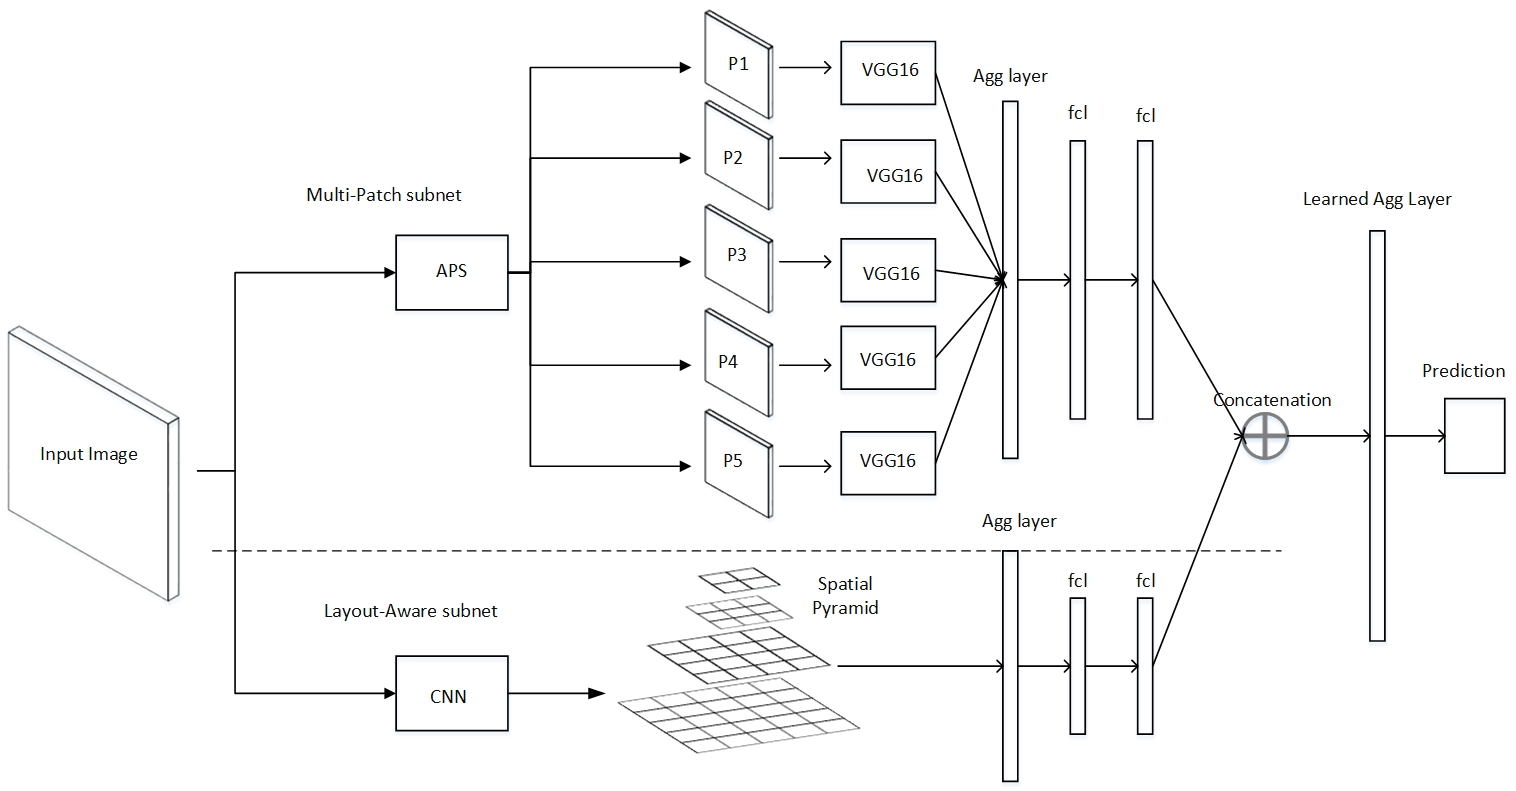
\includegraphics[scale=0.26]{figures/whole_net.jpg}
	\label{whole_net}
	\caption{The architecture of the A-Lamp}
\end{figure}

The architecture of our proposed A-Lamp is showed in Fig. \ref{whole_net}. Given an arbitrary sized image, multiple patches are carefully selected by the \textit{adaptive patch selection} module, and are fed into the \textit{Multi-Patch subnet}. A statistic aggregation layer is followed to effectively combine the extracted features from these multiple patches.
At the same time, a trained CNN is adopted to detect objects in the image. The local and global layout of the input image are further represented by an attribute-graph. At the end, a learned aggregation layer is utilized to incorporate the hybrid deep features from the two subnets and finally give the aesthetic prediction. More details will be illustrated in this section. 

\subsection{Multi-Patch subnet}

\begin{figure*}
	\centering
	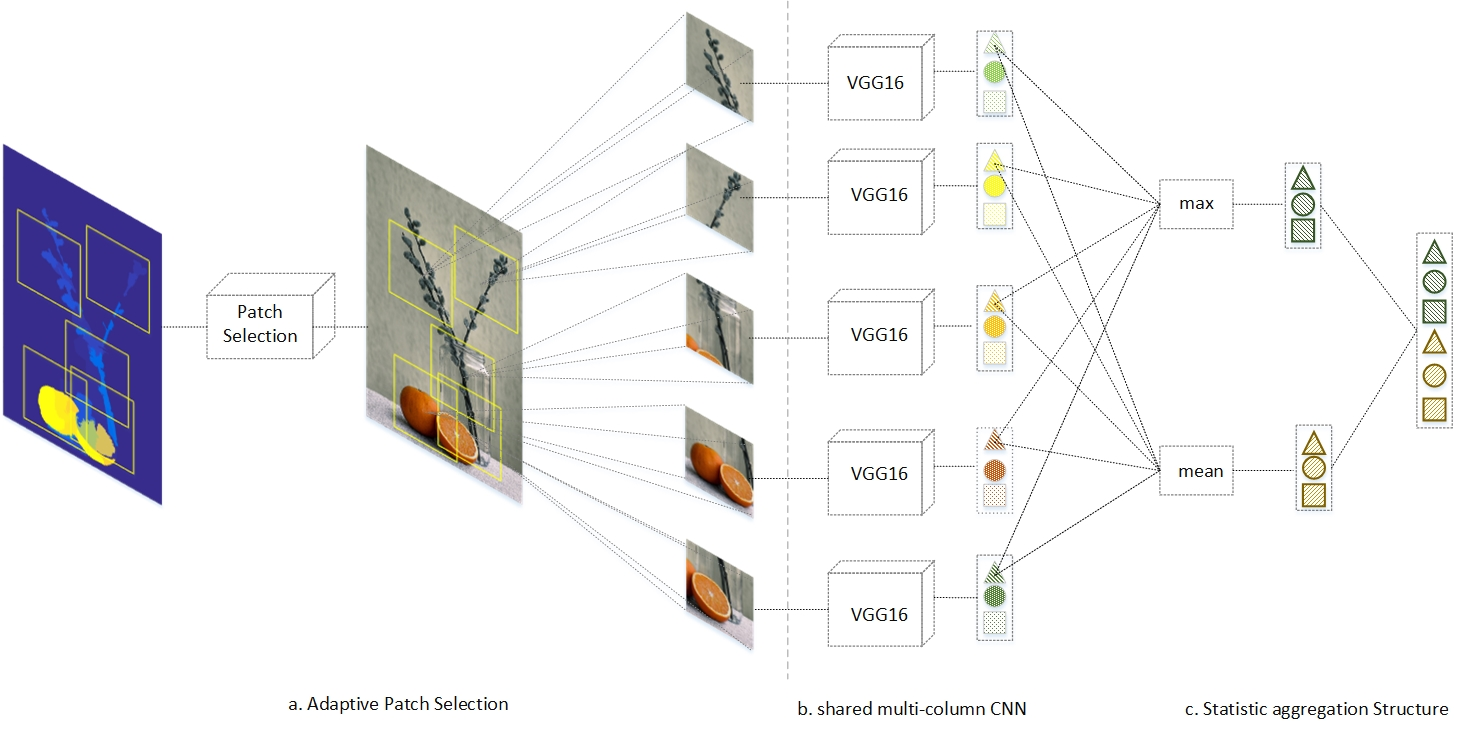
\includegraphics[scale=0.35]{figures/multi_patch_subnet.jpg}
	\label{multi_patch}
	\caption{The Multi-Patch subnet}
\end{figure*}

To support training from fine-grained details, we represent each image with a set of carefully cropped patches, and associate the set with the image's label.
The training data is ${{\rm{\{ }}{{\rm{P}}_n}{\rm{, }}{{\rm{y}}_n}{\rm{\} }}_{n \in [1,N]}}$, where ${P_n} = {\{ {p_{nm}}\} _{m \in [1,M]}}$ is the set of $M$ patches cropped from each image. 
As shown in Fig.\ref{multi_patch}, the Multi-Patch subnet contains mainly three parts: an adaptive patch selection module, a set of paralleled CNNs that are used for extracting deep features from each of the patch, and an orderless aggregation structure which combines the extracted deep features from the multi-column CNNs jointly.

\subsubsection{Adaptive Patch Selection}
Instead of randomly cropping 50 sets of patches (totally 250 patches for each image) \cite{Lu:2015:ICCV}, we aim to carefully select the most discriminative and informative patches to enhance training efficiency. To realize that, we studied professional photography rules and human visual principles. 
We find that human visual attention does not distribute evenly within an image.
That means, some regions play more important roles when people valuating
photos, while the others do not. 

In addition, holistic analysis is critical 
for evaluating an image's aesthetics. Thus just focus on the subjects is not enough for aesthetic assessment. Therefore, several issues are concerned when we perform patch selection:

\textbf{Saliency Map} The task of saliency detection is to identify the most important and informative part of a scene. Saliency map models human visual distribution, and is capable of highlighting visually attention region. Therefore, it is natural to adopt saliency map for selecting regions that human pay much more attention to.

\textbf{Pattern Diversity} Despite that, we also encourage diversification within a set of patches. Different from some conventional computer vision tasks (e.g. image classification and object recognition) which just need to focus on the foreground objects. To evaluate image aesthetics, holistic analysis is critical. Because some important aesthetic characters, e.g. Low-of-Depth, color harmonization, simplicity, etc., are perceived by analyzing both the foregroud and the background as a whole. 
%As wen can see from Fig. \ref{intro}, the foreground objects 
%(bird and flower) and the background are show in different patterns. Such different patterns represent the most distinguish parts within an image, which are critical clues for us to detect these global aesthetic properties. 

\textbf{Overlapping Constraint} Spatial distance for each patch pair is considered to constrain the overlapped ratio of these selected patches. 

Therefore, we formulate the patch selection as an optimization problem.  An objective function is defined to search for the optimal combination of patches:
\begin{equation}
\{ {c^ * }\}  = \mathop {argmax}\limits_{i,j \in [1,M]} \left[ {\sum\limits_{i = 1}^M {{S_i}}  + \sum\limits_{i \ne j}^M {{D_p}({{\widetilde {\rm N}}_i},{{\widetilde {\rm N}}_j}) + \sum\limits_{i \ne j}^M {{D_s}({c_i},{c_j})} } } \right]
\end{equation}
where ${\{ c_m^ * \} _{m \in [1,M]}}$ is the optimal set of $M$ selected patches centers.
where $\{ {c^ * }\} $ is the optimal subset of selected patch centers. $\;{S_i} = \frac{{sal({p_i})}}{{area({p_i})}}$ is the normalized saliency value that 
each patch $p_i$ occupies. The saliency value is obtained by a graph-based saliency detection approach \cite{C.Yang:2013:CVPR:graph_based_saliency}.
${D_p}( \cdot )$ is the pattern distance function which 
measures the difference of two patches' patterns. 
Here we adopt edge and chrominance distribution to represent the pattern of each patch. To measure the difference of edge distribution of each patch pairs, we model the edge and chrominance distribution of a patch using a multi-variant Gaussian. ${{\tilde N}_m} = {\{ {N_e}({\mu _e},{\sum _e}),{N_c}({\mu _c},{\sum _c})\} _{m \in [1,M]}}$ denotes the edge distribution ${N_e}({\mu _e},{\sum _e})$ and chrominance distribution ${N_c}({\mu _c},{\sum _c})$ of patch $p_m$. We formulate the problem by mapping these distribution to the \textit{Wasserstein Metric space} $M_{M\times M}$. The we define the $p^{th}$ \textit{Wasserstein distance} between the distribution  ${{\tilde N}_i}$ and ${{\tilde N}_j}$ as:
\begin{equation}
{D_p}({{\tilde N}_i},{{\tilde N}_j}) = {\left( {\mathop {\inf }\limits_{r \in \Gamma ({{\tilde N}_i},{{\tilde N}_j})} \int_{M \times M} {d{{(x,y)}^p}d\gamma (x,y)} } \right)^{1/p}}
\end{equation}
${D_s}( \cdot )$ is the spatial distance function, which is measured by Euclidean Distance.

\subsubsection{Orderless Aggregation Structure}
We perform aggregation of the multiple instances to support our network learn from multiple patches cropped from the original image.
Let ${\left\langle {{\rm{Blo}}{{\rm{b}}_n}} \right\rangle _{l}} = \{ b_i^n\} _{i \in [1,M]}^{l}$ be the set of patch features extracted from $n_{th}$ image 
at $l_{th}$ layer of the shared CNNs. Where $b_i^n$ is a $K$ dimensional vector.
$T_k$ denotes the set of values of the $k_{th}$ component of all ${b_i} \in Blob$, i.e. ${T_k} = {\{ {d_{ik}}\} _{i \in [1,M]}}$.

The orderless aggregation layer is comprised of a collection of statistical functions, 
i.e., ${F_{Agg}} = {\{ F_{Agg}^u\} _{u \in [1,U]}}$. Each $F_{Agg}^u$ computes
$Blob$ returned by the shared CNNs. In our work, we propose to have $U = \{ max,\;mean\} $. 
The outputs of the functions in $U$ are concatenated to produce a ${K_{stat}}$-dimensional feature vectors. Two fully connected layers are followed for implementing of multi-patch
aggregation component. The whole structure can be expressed as a function 
$f:\{ Blob\}  \to {{{K_{stat}}}}$:
\begin{equation}
f(Blob) = W \times ( \oplus _{u = 1}^U \oplus _{k = 1}^KF_{Agg}^u({T_k}))
\end{equation}
where $ \oplus$ is a vector concatenation operator which produces a column vector, $W \in {^{{K_{stat}} \times UK}}$ is the parameters of the fully-connected layer. 
Fig. \ref{multi_patch} shows an example of Statistics Aggregation Structure with $M = 5$ and $K=3$. In practice, the feature dimension $K=4096$.

\subsection{Layout-Aware Subnet}
The layout of an image is another critical ingredient that
affecting aesthetics. Good and balanced composition could make an 
image look more appealing even if the scene being shot is normal. 
In this paper, we develop a novel Layout-aware subnet, and combine it with the Multi-Patch subnet to effectively enhance the performance of our proposed A-Lamp CNN. To effectively represent image layout, we construct \textit{Attribute-graph}, which is an undirected fully connected graph, incorporating both local and global image characteristics. As can be seen from Fig. \ref{layout}, the graph nodes characterize salient objects as well as the overall scene context using node attributes,  while the edges capture the object topology. 

\begin{figure*}
	\centering
	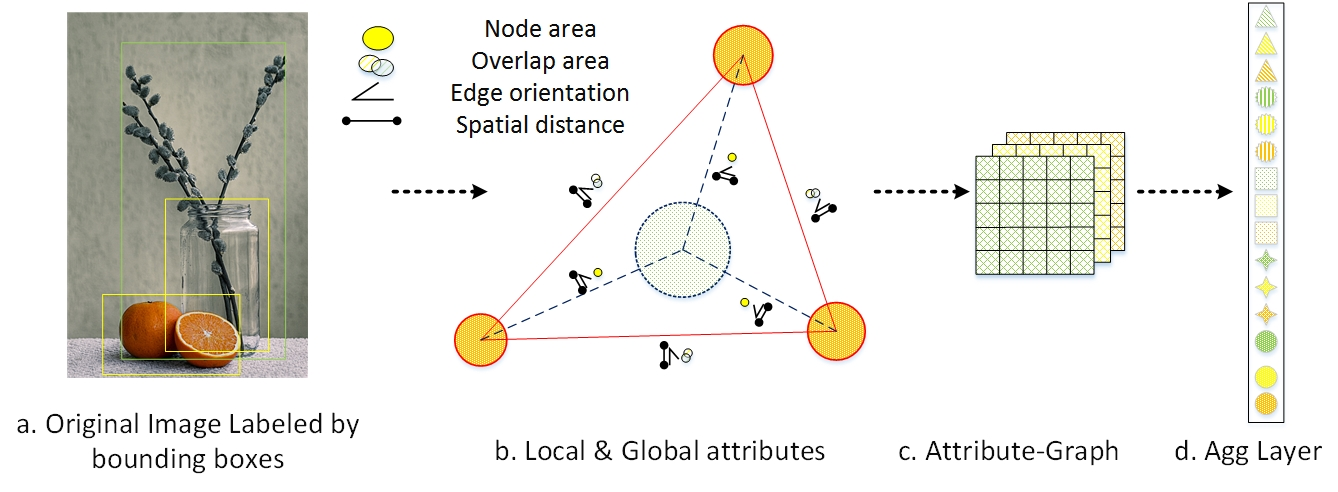
\includegraphics[scale=0.45]{figures/layout_graph.jpg}
	\label{layout}
	\caption{Architecture of the Layout-Aware subnet}
\end{figure*}

We first employ a trained CNN  \cite{zhang:2015:CVPR:boundingbox} to localize the salient objects. Let ${\rm I}:{\{ {{\rm B}_i},{s_i}\} _{{N_{obj}}}}$ denotes a set of detected objects in image ${\rm I}$, where each object is labeled by a bounding box ${{\rm B}_i}$ and associated with a confidence score ${s_i}$, $N_{obj}$ denotes the number of objects.
Here $G(V,E)$ is an undirected fully connected graph. 
$V = \{{V_{local}},{V_{global}}\}$ represents the nodes and $E$ represents the set of edges connecting the nodes. Each object present in the image contributes to a graph node resulting in a total of $N_{obj}$ local nodes ${V_{local}} = \{ {v_1}, \cdot  \cdot  \cdot ,{v_{{N_{obj}}}}\} $. The global node $V_{global}$ represents the background. An image with $N_{obj}$ objects is thus transformed into a graph having $N_{obj}+1$ nodes. We define two kind of edges, i.e. local edges and global edges. Where local edges refer to the edges between two local nodes, there will be $({N_{obj}} - 1)!$ such edges. The edges connecting local nodes and global node are global edges, there will be $N_{obj}$ such edges.

Each local node is represented using local attributes. These local attributes are limited to the area occupied by the bounding box of that particular object. The global node captures the overall essence of the image. The features of the model are defined so as to capture the spatial configuration of the image components. The local features capture the relative arrangement of the objects with respect to each other while the global features define the positioning of the objects in the image. The features are represented by 
\begin{equation}
f({e_{ij}}) = \left\{ {\begin{array}{*{20}{c}}
	{[{\mu _{ij}},\;{\theta _{ij}},\;{o_{ij}}]\;\;\;\;\;\;\;\;\;if\;{v_i},{v_j} \in {V_l}}\\
	{[{\mu _{ig}},\;{\theta _{ig}},\;area({v_i})]\;\;\;\;\;if\;{v_i} \in {V_l}\;\& {v_j} = {V_g}}
	\end{array}} \right.
\end{equation}
$e_{ij}$ represents the edge connecting node $v_i$ to node $v_j$. $\mu_{ij}$ is the spatial distance between object centroids. $\theta_{ij}$ represents the angle of the graph edge with respect to the horizontal taken in the anti-clockwise direction. It indicates the relative spatial organization of the two objects. $o_{ij}$ represents the amount of overlap between the bounding boxes of the two objects and is given by 
\begin{equation}
{o_{ij}} = \frac{{area({v_i}) \cap area({v_j})}}{{\min (area({v_i}),area({v_j}))}}
\end{equation}
where ${area({v_i})}$ is the fraction of the image area occupied by the ${i^{th}}$ bounding box.
The intersection of the two bounding boxes is normalized by the smaller of the bounding boxes to ensure the overlap score of one, when a smaller object is inside a larger one. $\mu_{ig}$ and $\theta_{ig}$ are the magnitude and orientation of the edge connecting the centroid of the object corresponding to node $v_i$ to the global centroid. The global centroid is computed by:
\begin{equation}
{c_g} = \frac{1}{N}\sum\limits_{k = 1}^N {{c_k}}
\end{equation}
where $c_k$ represents the centroid of the $k^{th}$ local node. The global centroid represents the center of the geometrical layout of the objects in the image. The edges connecting each object to the global node illustrate the placement of that object with respect to the overall object topology.

The architecture of our proposed \textit{Layout-Aware subnet} is shown in Fig. \ref{layout}. As we can see, an aggregation layer is adopted to concatenate the constructed attribute graphs into a feature vector ${\vec \nu }$, and further combined with the \textit{Multi-Patch subnet}, which can be seen in Fig. \ref{whole_net}. By statistical study, we find that, the confidence score is very low when ${N_{obj}} \ge 5$. Therefore, we set $N_{obj} = 4$ to fix the dimension of the feature vector ${\vec \nu }$.

\section{Implementation Details}
In our implementation, we simplify the computational complexity and release the memory burden in training by first training the Multi-Patch subnet and then combining the layout-aware subnet to fine-tune A-Lamp. 
The weights of multiple shared column CNNs in the Multi-Patch subnet are initialized by the weights of VGG16 which is pre-trained on the ImageNet \cite{Alex:2012:NIPS:ImageNet}. VGG16 is one of the state-of-the-art object-recognition networks that has been adopted with great success to many different computer vision problems. 
Following \cite{Lu:2015:ICCV}, The number of patches in a bag is set to be 5. The patch size is fixed to be 224 $ \times 224 \times 3$. The base learning rate is 0.01, the weight decay is 1e-5 and momentum is 0.9.  
All the network training and testing are done by using the Caffe deep learning framework\cite{Jia:2014:ACMMM:caffe}. The networks are trained with the Adam. 

\section{Experiments} \label{experiments}
We systematically evaluate our method on the AVA dataset \cite{Murray:MMP2012:AVA}, which, to our best knowledge, is the largest publicly available aesthetic assessment dataset. The AVA dataset provides about 250,000 images in total. The aesthetics quality of each image in the dataset was rated on average by roughly 200 people with the ratings ranging from one to ten, with ten indicating the highest aesthetics quality. For a fair comparison, we use the same partition of training data and testing data as the previous
work \cite{Lu:2014:ACMMM,Lu:2015:ICCV,Mai:2016:CVPR,Murray:MMP2012:AVA} ( roughly 20,0000 images for training and 19,000 images for testing). We also follow the same procedure as the previous work to assign a binary aesthetics label to each image in the benchmark. Specifically, images with mean ratings smaller than equal to 5 are labeled as low quality and those with mean ratings larger than 5 are labeled as high quality. 

\subsection{Comparison with the state-of-the-art}
We denote our \textit{Multi-Patch subnet} as \textbf{Ours-MP-Net} and \textit{Layout-Aware Multi-Patch CNN} as \textbf{A-Lamp}. To evaluate the proposed approach, both \textbf{Ours-MP-Net} and \textbf{A-Lamp} are compared with several state-of-the-arts in this section.

\subsubsection{Analysis of adaptive Multi-Patch subnet}
For a fair comparison, we first perform training and testing only using our proposed Multi-Patch subnet, and evaluate Ours-MP-Net with the Deep Multi-Patch-Aggregation Network(DMA-Net) in \cite{Lu:2015:ICCV}. DMA-Net is a very recent dedicated deep Multi-Patch CNN for aesthetic assessment.
Specifically, DMA-Net performs multi-column CNN training and testing. Five randomly cropped patches from each image was used as training, and the label of the image is associated with the bag of patches. DMA-Net{\tiny ave} and DMA-Net{\tiny max} train deep multi-patch aggregation network using standard patch pooling scheme, where DMA-Net{\tiny ave} performs average pooling and DMA-Net{\tiny max} performs max pooling. The DMA-Net using Statistics Aggregation Structure as DMA-Net{\tiny stat} and Fully-Connected Sorting Aggregation Structure as DMA-Net{\tiny fc}. 

\begin{table}
	\begin{center}	
		\begin{tabular}{||c|c||} 
			\hline
			Method & Accuracy \\
			\hline\hline
			DMA-Net{\tiny ave} & 73.1 $\%$ \\
			DMA-Net{\tiny max} & 73.9 $\%$ \\
			DMA-Net{\tiny stat} & 75.4$\% $ \\
			DMA-Net{\tiny fc} & 75.4$\% $ \\
			\hline
			\textbf{Ours-MP-Net} & \textbf{81.7$\% $}\\
			\hline
		\end{tabular} \label{tabel1} 
	\end{center} 
\caption{Performance of Multi-Patch subnet}
\end{table}

The results are shown in Table \ref{tabel1}. We can see that, our methods outperform all kinds of DMA-Net architectures.
Although \cite{Lu:2015:ICCV} randomly copped 50 groups of patches, which takes totally 250 patches for each image, and trained the DMA-Net for 50 epochs. The random cropping strategy may lost much useful information and made the training data confusing for network. Instead of random cropping, we adaptively select the most informative and discriminative patches as input, which shows great improvement. From Fig.\ref{intro}, we can see that, the salient objects, i.e. the bird and the flower, are selected. Within these patches, the most important information and the fine-grained details are remained. Despite that, the background, i.e. the blue sky and the green ground, are also selected so that global characteristics, e.g. color harmony, Low-of-Depth, can be learned. More examples of selected patches are shown in Fig. \ref{patches}. We can see that, our strategy is not only effective in selecting the most salient regions (e.g. the human's eyes and face, the orange flowers, etc.), but also capable of encouraging the pattern diversity (e.g. the green leaf and green beans, the flower and the gray wall).
What's more, our adaptive patch selection strategy much enhanced the training efficiency. The result of Ours-MP-Net is obtained by taking 20-30 training epochs, which is much less than 50 epochs in \cite{Lu:2015:ICCV}, while showing better performance.
The reason of higher accuracy may also lies in different CNN architecture we used. \cite{Lu:2015:ICCV} adopt shallow CNN, which has only 4 convolution layers and followed by two fully connected layers. We use VGG16 \cite{Simonyan14c:2014:VGG}, which shows significant improvement.

\begin{figure*}
	\centering
	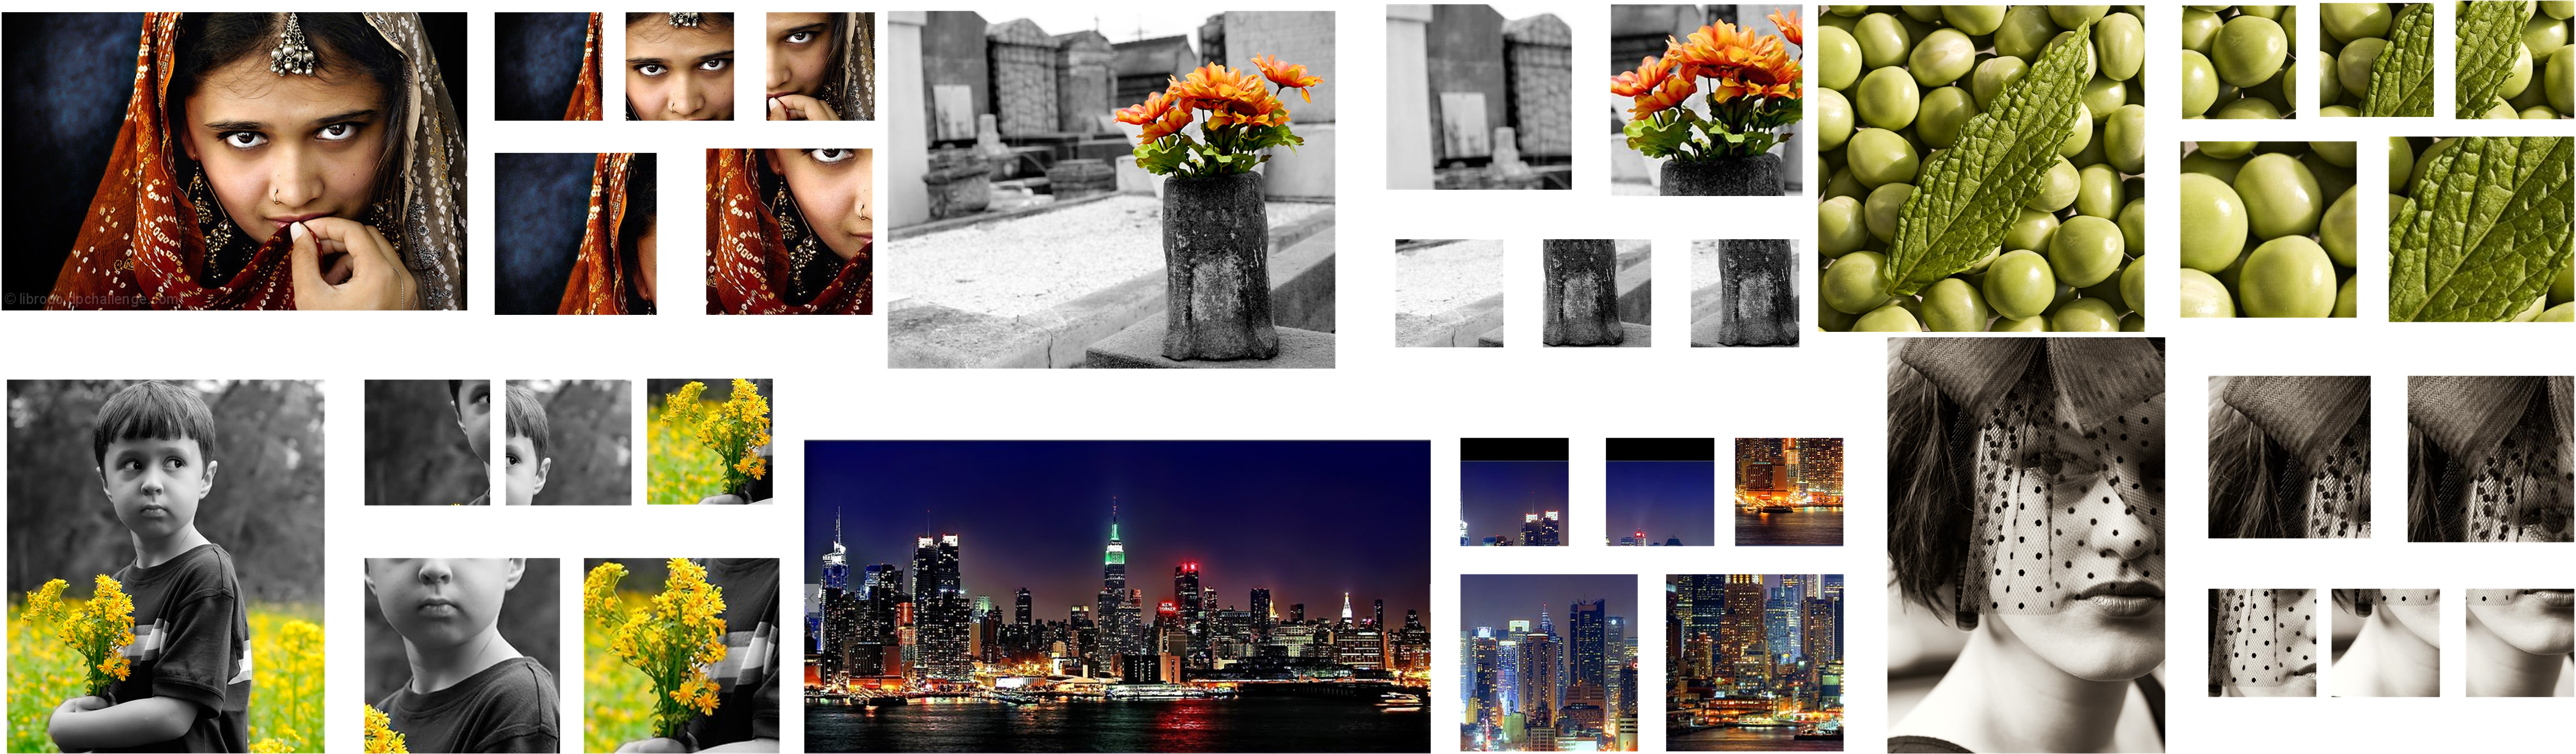
\includegraphics[scale=0.15]{figures/patch_selection.jpg}
	\label{patches}
\end{figure*}

\subsubsection{A-Lamp CNN Performance}

\begin{table}
	\begin{center}
		\begin{tabular}{||c|c|c||} 
			\hline
			Method & Accuracy & F-measure\\
			\hline\hline
			AVA & 67.0 $\%$ & na  \\
			VGG-Crop & 71.2 $\%$ & 0.83 \\
			VGG-Scale & 73.8 $\%$ & 0.83 \\
			VGG-Pad & 72.9 $\%$ & 0.83 \\
			\hline
			SPP-CNN & 76.0 $\%$ & 0.84 \\
			MNA-CNN & 77.1 $\%$ & 0.85 \\
			MNA-CNN-Scene & 77.4 $\%$ & $N{A^ * }$ \\
			SCNN & 71.2 $\%$ & $N{A^ * }$ \\
			DCNN & 73.25 $\%$ & $N{A^ * }$ \\
			DMA-Net-ImgFu & 75.4 $\%$ & $N{A^ * }$\\
			\hline\hline
			\textbf{Ours-MP-Net} & \textbf{81.7$\% $} & \textbf{0.91} \\
			\textbf{A-Lamp} & \textbf{82.5 $\%$} & \textbf{0.92} \\
			\hline
		\end{tabular} \label{tabel2}
	\end{center}
\caption{A-Lamp CNN performance comparisons with the state-of-the-art}
\end{table}


\begin{figure}
	\centering
	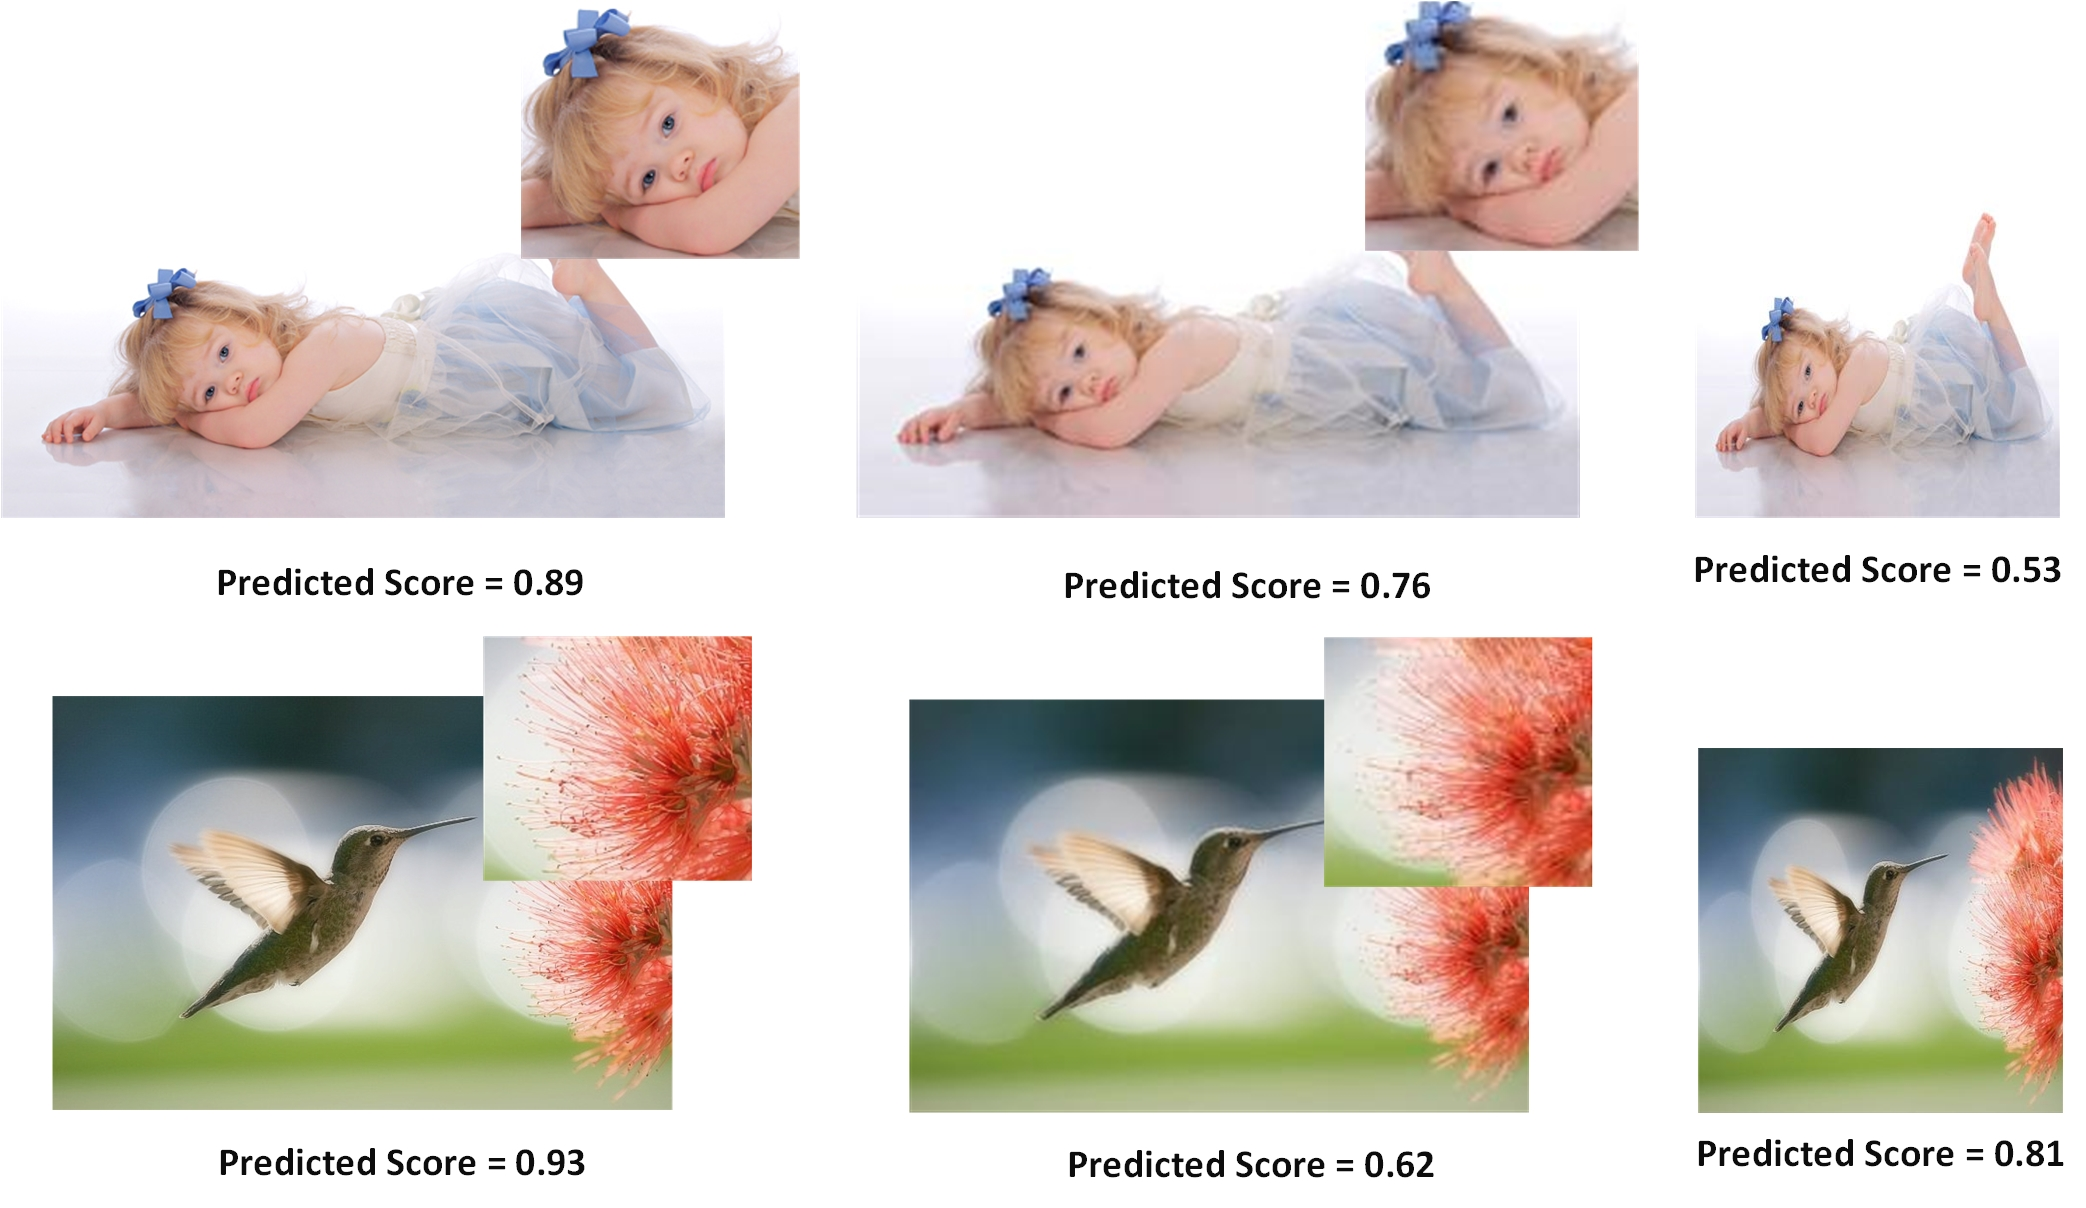
\includegraphics[scale=0.18]{figures/expr_transform.jpg}
	\label{trans_img}
\end{figure}

Table \ref{tabel2} reports results of our A-Lamp CNN on the AVA dataset for image aesthetics categorization. AVA \cite{Murray:MMP2012:AVA} provides the state-of-the-art result for methods that use manually designed features and generic image features for aesthetics assessment. It is obvious that, all the deep CNN methods outperformed the conventional approach.

To examine the effectiveness of our proposed methods, we compare Ours-MP-Net and A-Lamp with the baseline methods which take fixed-size inputs. In particular, we experiment with three VGG16-based aesthetics assessment methods, each operating on a different type of transformed input.

VGG16-Crop: The input of the network is obtained by randomly cropping from the original image with a 224$\times$224 cropping window. This cropping window size is the fixed size required by the VGG16 architecture. During training, we extract five random crops for each image in the training
set and train the network on all the crops with their corresponding
aesthetics labels. For each testing image, we follow the previous work \cite{Lu:2015:ICCV} to predict the aesthetics quality for 50 random crops obtained from the image and take their average as the final prediction result.

VGG16-Scale: The input of the network is obtained by scaling
the original input image to the fixed size of 224$\times$224. Both training and testing are conducted on the scaled version of the input images.

VGG16-Pad: The original image is uniformly resized such that the larger dimension becomes 224 and the aspect ratio is preserved. The 224$\times$224 input is then formed by padding the remaining dimension of the transformed image with zero pixels.

We can see that, both our proposed Multi-Patch subnet and the A-Lamp net outperforms these fixed-size input VGG nets. Such results confirmed that training network on multiple patches generates better prediction performance than networks training on a single patch.

We also compared our work with some latest non-fixed-size restriction methods, i.e. SPP-CNN \cite{He:archive:2014} and MNA-CNN \cite{Mai:2016:CVPR}.  Different from these methods that train from several different level of scaled images, we implement the A-Lamp network to be trained from original images. The result turns out learning from original images is critical for aesthetic assessment, as discussed in \ref{intro}. In addition, higher prediction accuracy further proves that, our proposed adaptive Multi-Patch strategy is more efficient than the spatial pooling layers adopted in SPP-CNN and MNA-CNN.

To show the effectiveness of our proposed layout-aware subnet, we compare A-Lamp with several latest deep CNN networks that incorporate global information for learning. MNA-CNN-Scene \cite{Mai:2016:CVPR} replace the average operator in the MNA-CNN network with a new aggregation layer that takes the concatenation of the sub-network predictions and the image scene categorization posteriors as input and output the final aesthetics prediction. We can see that, the performance not show much improvement after incorporating with scene attributes. 

DCNN is a double column convolutional neural network, which allows network
training using two inputs extracted from different spatial scales of one image.
Specifically, \cite{Lu:2014:TMM:rating} combine random cropped and wrapped images as inputs to train the proposed double-column network. By comparing our A-Lamp test accuracy (82.5 $\%$) with DCNN (73.25 $\%$), we observe that using random cropped and wrapped image to capture local and global image characters is not as effective as our approach.  

DMA-Net-ImgFu remains the global view of the entire image \cite{Lu:2015:ICCV} by leveraging pre-trained models with external data (e.g., ImageNet features). The result of DMA-Net-ImgFu (75.4 $\%$) is obtained by averaging the prediction results of DMA-Net and the fine tuned Alexnet \cite{Alex:2012:NIPS:ImageNet}. It is interesting that, though \cite{Lu:2015:ICCV} incorporated transformed entire images to represent global information, it still fall behind the performance of our proposed A-Lamp (82.5 $\%$). Such results further validate the effectiveness of our proposed layout-aware subnet. The layout-aware approach slightly boosts the performance of Ours-MP-Net, and significantly performs better than the other state-of-the-art approaches. Such results show that both the holistic layout information and fine-grained information are useful for image aesthetics categorization, and the proposed adaptive Multi-Patch selection approach captures the fine-grained information in compensate to the global view of images. 


\begin{figure} [!t]
	\centering
	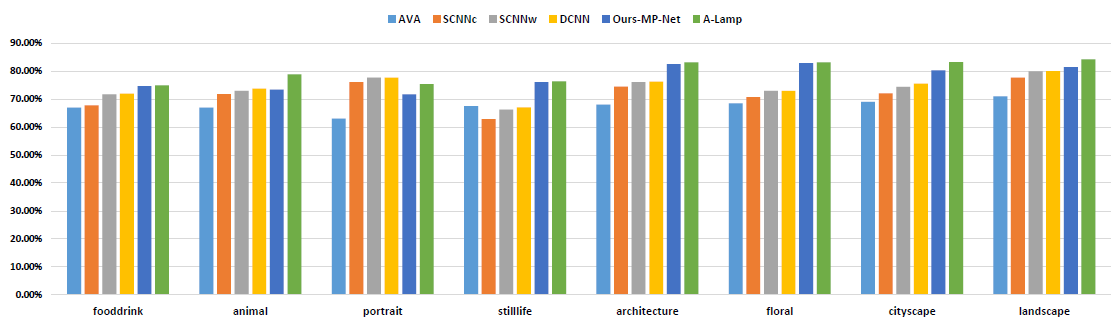
\includegraphics[scale=0.3]{figures/category.jpg}
	\label{category}
\end{figure}

\begin{figure*} [!t]
	\centering
	\includegraphics[scale=0.1]{figures/samples.jpg}
	\label{samples}
\end{figure*}

We further examined if our A-Lamp network has learned to respond to the change in image holistic layout and fine-grained details. To test this, we random collect 20 high-quality images from the AVA dataset. We generate a down sampled version and a wrapped version from the original image. As seen in Fig. \ref*{trans_img}, the down-sampled version remains the same aspect ratio (i.e. the layout has not be changed), while half of the original dimension. The wrapped version is generated by scaling along the longer edge to make it square. From the predicted aesthetic score we can notice that, our A-Lamp net give higher score than both the transformed versions. 
Fig. \ref*{trans_img} shows examples used in the study and their transformed versions, along with our A-Lamp predicted posteriors. The result shows that our A-Lamp is able to reliably respond to the change of image layout and fine-grained details caused by transformation. In addition, we can notice that when the image content is more semantic, it will be sensitive to holistic layout, as we can see, the wrapped version of the portrait photo is much lower than the original and even down-sampled one. It is interesting that the wrapped version for the second photo seems not so bad, while the down-sampled version falls a lot due to much detail loss. To further investigate the effectiveness our A-Lamp networks adaption for content-based image aesthetics, we performed content-based photo aesthetic analysis in the next section \ref{content}.



\subsection{Content-based photo aesthetic analysis} \label{content}
We took the eight most popular semantic tags, i.e. portrait, animal, still-life, food-drink, architecture, floral, cityscape and landscape, as used in \cite{Murray:MMP2012:AVA}. We used the same testing image collection with \cite{Lu:2014:TMM:rating}, roughly 2.5K for testing in each of the categories.
In each of the eight categories, we systematically compared
Ours-MP-Net and A-Lamp net with baseline approach \cite{Murray:MMP2012:AVA} (denoted by AVA) and the state-of-the-art approach \cite{Lu:2014:TMM:rating}. Specifically, SCNN{\tiny c} and SCNN{\tiny w} denote the single-column CNN in \cite{Lu:2014:TMM:rating} that takes center-cropping and warpping as inputs, respectively. DCNN denotes the double-column CNN in \cite{Lu:2014:TMM:rating}.
As presented in Fig. \ref*{category}, the proposed networking training approach significantly outperforms the state-of-the-art in most of the categories, where "floral" and "architecture" show much improvements. We find that, photos belonging to these two categories often show complicated texture details, which can can be seen in Fig. \ref{samples}. The proposed adaptive Multi-Patch subnet remains the fine-grained details, thus turns out much better performance. We also find that A-Lamp show much better performance than Ours-MP-Net in "portrait" and "animal". This result indicates that once an image is associated with an obvious semantic meaning, then the global view is more important than the local view in terms of assessing image aesthetics. Fig.\ref{samples} shows some examples of the test images that are considered of the highest and lowest aesthetics values by our A-Lamp. Here we picked good photos from all of the eight categories.

\section{Conclusion}
This paper presents an Adaptive Layout-Aware Multi-Patch Convolutional Neural Network (A-Lamp CNN) architecture for photo aesthetic assessment. This novel scheme is able to accept arbitrary sized images, and deal with both fined grained details and holistic image layout simultaneously. To support A-Lamp training on these hybrid inputs, we extend the method by developing a dedicated double-subnet neural network structure, i.e. a Multi-Patch subnet and a Layout-Aware subnet. We further construct an aggregation layer to effectively combine the hybrid features from these two subnets. Our experiments on the large-scale AVA benchmark show that our A-Lamp CNN can significantly improve the state of the art in photo aesthetics assessment.
-----------------------------------------------------------------------

\cleardoublepage
{\small
	\bibliographystyle{IEEE}
	\bibliography{test}
}

\end{document}
